\documentclass[12pt, letterpaper]{article}

\usepackage[utf8]{inputenc}
\usepackage{systeme}
\usepackage{amsmath}
\usepackage{amssymb}
\usepackage{enumitem}
\usepackage{amsfonts}
\usepackage{amsthm}
\usepackage{graphicx}
\usepackage[colorinlistoftodos]{todonotes}
\usepackage{pifont}
\usepackage{mdframed,color}
\usepackage[left=3cm, right=3cm, top=3cm]{geometry}
\newcommand{\Z}{\mathbb{Z}}
\newcommand{\N}{\mathbb{N}}
\newcommand{\C}{\mathbb{C}}
\newcommand{\Q}{\mathbb{Q}}
\newcommand{\R}{\mathbb{R}}
\newcommand{\F}{\mathbb{F}}
\newtheoremstyle{statement}{3pt}{3pt}{}{}{\bfseries}{:}{.5em}{}

\theoremstyle{statement}
\newtheorem*{atmProp}{Proposition}

\newenvironment{atmProof}{\noindent\ignorespaces\paragraph{Proof:}}{\hfill \ding{122}\par\noindent}

\newcount\arrowcount
\newcommand\arrows[1]{
        \global\arrowcount#1
        \ifnum\arrowcount>0
                \begin{matrix}
                \expandafter\nextarrow
        \fi
}

\newcommand\nextarrow[1]{
        \global\advance\arrowcount-1
        \ifx\relax#1\relax\else \xrightarrow{#1}\fi
        \ifnum\arrowcount=0
                \end{matrix}
        \else
                \\
                \expandafter\nextarrow
        \fi
}

\title{Mastery Homework 2}
\author{Rafael Laya}
\date{Fall 2018}

\begin{document}
    \maketitle

    \section*{Section 1.5}
        \subsection*{Problem 26.} 
            \begin{atmProp}
                Suppose $A\Vec{x} = \Vec{b}$ has a solution. Explain why the solution is unique precisely when $A\Vec{x}= \Vec{0}$ has only the trivial solution.
            \end{atmProp}
            
            This is true, since when $A\vec{x}=\vec{0}$ has a non-trivial solution $\vec{\lambda}$ then we can find a solution $\vec{x_1} + \vec{\lambda}$ (where $\vec{x_1}$ is a solution to $A\vec{x}=\vec{b}$) to the equation $A\vec{x}=\vec{b}$ which contradicts the assumption.
            
            \begin{atmProof}
                Suppose $A\Vec{x}=\Vec{b}$ has atleast two distinct solutions $\Vec{x_1}, \Vec{x_2}$
                Suppose also that $A\Vec{x}=\Vec{0}$ has only the trivial solution. Then: 
                \begin{align*}
                    A(\Vec{x_1} - \Vec{x_2}) & = A\Vec{x_1} - A\Vec{x_2} \\
                    & = \Vec{b} - \Vec{b} \\
                    & = \Vec{0}
                \end{align*}
                Therefore $A\Vec{x} = \Vec{0}$ has a non-trivial solution (since $\vec{x_1}, \vec{x_2}$ are distinct) which contradicts our hypothesis. By contradiction $A\Vec{x} = \Vec{b}$ can only have one solution (not none either by assumption).
                
                Now suppose $A\Vec{x} = \Vec{0}$ has a non-trivial solution $\Vec{\lambda} = \begin{bmatrix} \lambda_1 \\ \vdots \\ \lambda_n \end{bmatrix}$ and $A\Vec{x} = \Vec{b}$ only has one solution $\Vec{x_1}$ then:
                
                \begin{align*}
                    A(\Vec{x_1} + \Vec{\lambda}) & = A\Vec{x_1} + A\Vec{\lambda} \\
                    & = \Vec{b} + \Vec{0} \\
                    & = \Vec{b} \\
                \end{align*}
                And since $\vec{\lambda}$ is not a trivial solution $\vec{\lambda} \neq \Vec{0}$ we have $\Vec{x_1} + \Vec{\lambda} \neq \Vec{x_1}$ so $A\Vec{x} = \Vec{b}$ has atleast two solutions which contradicts our hypothesis. By contradiction $A\Vec{x} = \Vec{0}$ must only have a trivial solution.
            \end{atmProof}
        
        \subsection*{Problem 28.}
            \begin{atmProp}
                If $\vec{b} \neq \vec{0}$, can the solution set of $A\vec{x}=\vec{b}$ be a plane through the origin? Explain.
            \end{atmProp}
            
                It cannot be the case, since if the solution set of $A\vec{x} = \vec{b}$ goes through the origin then $\vec{x} = \vec{0}$ must be a solution to the equation. However, $A\vec{0} = \vec{0}$ but $\vec{b} \neq \vec{0}$ therefore $\vec{x}= \vec{0}$ is not a solution to $A\vec{x} = \vec{b}$ and the solution set does not pass through the origin.
                
            \begin{atmProof}
                Suppose the solution set of $A\vec{x} = \vec{b}$ with $\vec{b} \neq \vec{0}$ is a plane through the origin, then $\vec{x} = \vec{0}$ is a solution to the equation. But:
                
                $$A\vec{x} = A\vec{0} = \vec{0} = \vec{b}$$
                
                This is a contradiction since $\vec{b} \neq \vec{0}$ by assumption. Therefore the solution set of $A\vec{x} = \vec{b}$ cannot be a plane through the origin with $\vec{b} \neq \vec{0}$
            \end{atmProof}
            
            \subsection*{Problem 38.}
            
            \begin{atmProp}
                Suppose $A$ is a 3x3 matrix and $\vec{y}$ is a vector in $\R^3$ such that the equation $A\vec{x} = \vec{y}$ does not have a solution. Does there exist a vector $\vec{z}$ in $\R^3$ such that the equation $A\vec{x}=\vec{z}$ has a unique solution?.
            \end{atmProp}
            
            No, there does not exist such a vector $\vec{z}$. Because $A\vec{x} = \vec{y}$ is inconsistent for some $\vec{y} \in \R^3$ then $\vec{y}$ must make a pivot column in the augmented matrix associated to the system and therefore $A$ has a row of zeros in its row reduced echelon form. $A$ has three rows and three columns (it is a 3x3 matrix) and since it has at least one row of zeros it must have at most 2 pivots and 2 basic variables and therefore at least one free variable. We can pick $\vec{z}$ in such a way that the system is inconsistent or consistent with infinite solutions, never with only one solution. 
            
            \begin{atmProof}
            Suppose $A$ is a 3x3 matrix and $\vec{y} \in \R^3$ is such that the equation $A\vec{x} = \vec{y}$ is inconsistent. Then, applying theorem 2 in our textbook we know that the right-most column of the augmented matrix $\begin{bmatrix} A && y\end{bmatrix}$ is a pivot column which is only possible if the matrix $A$ as a row of zeros in its row reduced echelon form. Therefore $A$ has at most 2 pivots (one per non-zero row) which means the equivalent system has at most 2 basic variables and at least 1 free variable. 
            Choose any $\vec{z} \in \R^3$ then the row reduced echelon form of the augmented matrix associated to $A\vec{x} = \vec{z}$, $\begin{bmatrix} A && \vec{z} \end{bmatrix}$ has either at least one row of the form $\begin{bmatrix} 0 && 0 && \dots && 0 && 1 \end{bmatrix}$ (when $\vec{z}$ forms a pivot column) and the system is inconsistent or the right-most column is not a pivot column and the system is consistent but then it has at least one free variable and the system has infinite solutions by the virtue of its free variables (guaranteed again by theorem 2).
            \end{atmProof}

        \section*{Section 1.6}
            \subsection*{Problem 12}
            \subsubsection*{a)}
            
            Assigning positive sign to the inflow of traffic at a node and negative sign to the outflow of traffic, we must have that the sum of inflows and outflows at a node is zero. This fact leads to the following equations: 
               
               
                 $\\\systeme* {
                x_1 - x_3 - x_4 - 40 = 0 ,
                -x_1 - x_2 + 200 = 0 ,
                x_2 - x_5 - 100 = 0 ,
                x_4 + x_5 = 60 
            }\\ $  
            
            
            or equivalently, 
            
            $\\
            \systeme* {
                x_1 - x_3 - x_4 = 40 ,
                x_1 + x_2 = 200 ,
                x_2 - x_5 = 100 ,
                x_4 + x_5 = 60 
            }      
            $
            
            Row reducing the augmented matrix associated to the system: 
            
            $$\begin{bmatrix}
            1 & 0 & -1 & -1 & 0 & 40 \\
            1 & 1 & 0  & 0  & 0 & 200 \\
            0 & 1 & 1  & 0  & -1 & 100 \\
            0 & 0 & 0  & 1  &  1 & 60 
            \end{bmatrix}
            \arrows4{}{R_2-R_1}{}{}
            \begin{bmatrix}
            1 & 0 & -1 & -1 & 0 & 40 \\
            0 & 1 & 1  & 1  & 0 & 160 \\
            0 & 1 & 1  & 0  & -1 & 100 \\
            0 & 0 & 0  & 1  &  1 & 60 
            \end{bmatrix}
            $$
            $$
            \arrows4{}{}{R_3-R_2}{}
            \begin{bmatrix}
            1 & 0 & -1 & -1 & 0 & 40 \\
            0 & 1 & 1  & 1  & 0 & 160 \\
            0 & 0 & 0  & -1  & -1 & -60 \\
            0 & 0 & 0  & 1  &  1 & 60 
            \end{bmatrix}
            \arrows4{}{}{-R_3}{}
            \begin{bmatrix}
            1 & 0 & -1 & -1 & 0 & 40 \\
            0 & 1 & 1  & 1  & 0 & 160 \\
            0 & 0 & 0  & 1  & 1 & 60 \\
            0 & 0 & 0  & 1  &  1 & 60 
            \end{bmatrix}$$
            $$
            \arrows4{R_1+R_3}{R_2-R_3}{}{R_4-R_3}
            \begin{bmatrix}
            1 & 0 & -1 & 0 & 1 & 100 \\
            0 & 1 & 1  & 0  & -1 & 100 \\
            0 & 0 & 0  & 1  & 1 & 60 \\
            0 & 0 & 0  & 0  &  0 & 0 
            \end{bmatrix}
            $$
            
            Then the system is solved:
            
            $\\
            \systeme* {
                x_1 - x_3 + x_5 = 100,
                x_2 + x_3 - x_5 = 100,
                x_4 + x_5 = 60
            }$ ; with $x_3, x_5$ free variables
            
            or
            
           $\\
            \systeme* {
                x_1 = 100 + x_3 - x_5,
                x_2= 100 - x_3 + x_5,
                x_4 = 60 - x_5
            }$ ; with $x_3, x_5$ free variables
            
            which is the general traffic flow assumming $x_1, x_2, x_3, x_4, x_5$ are non-negative.
            
            \subsubsection*{b)}
            When the road whose flow $x_4$ is closed then $x_4 = 0$ and by substitution $x_5 = 60$ 
            
            $\\
            \systeme* {
                x_1 = 40 + x_3,
                x_2= 160 - x_3,
                x_4 = 0,
                x_5 = 60
            }$ ; with $x_3$ free variable
            
            \subsubsection*{c)}
            When $x_4 = 0$ the minimum value of $x_1$ is $x_1 = 40$ cars per minute since the free variable $x_3$ has to be non-negative.

            \section*{Section 1.7}
            
            \subsection*{Problem 28}
            How many pivot columns must a 7x5 matrix $A$ have if its columns span $\R^5$? Why?
            
            $\\$In order for the columns of $A$ to Span $\R^5$, the augmented matrix associated $\begin{bmatrix} A && \vec{b}\end{bmatrix}$ must not have $\vec{b}$ as a pivot column. In other words, $A$ cannot have a row of zeros in its Row Reduced Echelon Form, because if it did, we could choose $\vec{b}$ so that there is a pivot in the rightmost column and the system would be inconsistent and therefore $\vec{b}$ is not in the Span of the columns of $A$. 
            
            \begin{atmProp}
            If matrix $A$ of 5x7 Spans all of $\R^5$, then it has five pivot columns.
            \end{atmProp}
            \begin{atmProof}
            Let $A$ be a matrix of 5x7 and suppose that its columns $\vec{a_1}, \dots, \vec{a_7}$ Span all of $\R^5$. The matrix $A$ has a $k$ non-negative integer amount of pivot columns. The matrix $A$ can only have as much as one pivot per column therefore $k \leq 5$. Suppose $k < 5$. Since $k < 5$ and $A$ has 5 rows, the Row Reduced Echelon Form of $A$ has at least one row of zeros. We can choose $\vec{b}$ such that the augmented matrix $\begin{bmatrix} A && \vec{b}\end{bmatrix}$ has a row of the form $\begin{bmatrix} 0 & \dots & 0 && 1\end{bmatrix}$ which implies the system $A\vec{x} = \vec{b}$ is inconsistent or equivalently $\vec{b} \notin \operatorname{Span}(\{\vec{a_1}, \dots, \vec{a_7}\})$ which is a contradiction to our hypothesis, so we are left with $k = 5$. $A$ has five pivot columns. 
            \end{atmProof}
            
            \subsection*{Problem 30}
            Fill in the blank in the following statement: "If $A$ is a mxn matrix, then the columns of $A$ are linearly independent if and only if $A$ has $\_\_\_\_\_\_\_$ pivot columns."
            b) Explain why the statement in (a) is true.
            
            \subsubsection*{a)}
            n pivot columns.
            \subsubsection*{b)}
            Consider $A$ with $n$ columns, $\vec{a_1}, \dots, \vec{a_n} \in \R^m$ and consider the equation:
            
            \begin{equation}
                x_1\vec{a_1} + \dots + x_n\vec{a_n} = \vec{0}
                \label{eq1}
            \end{equation}
            
            Suppose first the columns of $A$ are linearly independent, then the only solution to the equation above is $x_i = 0$ for $i = 1, \dots, n$. Suppose that $A$ has $k$ pivots, $k \leq n$ since $A$ can only have at most one pivot column per column. Now when $k < n$ the augmented matrix $\begin{bmatrix} \vec{a_1} & \dots & \vec{a_n} && \vec{0}\end{bmatrix}$ has $k < n$ column pivots that correspond to basic variables, therefore there must be at least one free variable (the system is consistent since $A\vec{x}=\vec{b}$ always has the trivial solution) and therefore there are infinitely many solutions which contradicts the our hypothesis that the columns of A are linearly independent. By contradiction we are left with $k=n$.
            
            Suppose now that $A$ has $n$ pivot columns. This implies that the first $n$ columns of the augmented matrix $\begin{bmatrix} \vec{a_1} & \dots & \vec{a_n} && \vec{0}\end{bmatrix}$ are pivot columns which correspond to basic variables and by theorem 2 in our textbook $A\vec{x}=\vec{b}$ has unique solution. This unique solution is the trivial solution $\vec{x}=\vec{0}$. Therefore the only solution to equation \ref{eq1} is $x_i = 0$ for $i=1,\dots,n$
            
            Therefore the columns of $A$ are linearly independent if and only if $A$ has $n$ pivot columns.
            
            \subsection*{Problem 38}
            
            \begin{atmProp}
            if $\vec{v_1}, \vec{v_2}, \vec{v_3}, \vec{v_4}$ are linearly independent vectors in $\R^4$, then $\{\vec{v_1}, \vec{v_2}, \vec{v_3}\}$ is also linearly independent.
            \end{atmProp}
            
            \begin{atmProof}
            Suppose the set $\{\vec{v_1}, \dots, \vec{v_4}\}$ is a linearly independent set, then:
            
            \begin{equation}
                x_1\vec{v_1} + x_2\vec{v_2} + x_3\vec{v_3}+ x_4\vec{v_4} = \vec{0}
                \label{eq:2}
            \end{equation}
            
            Has unique solution $x_1=x_2=x_3=x_4=0$. Now consider the special case when $x_4=0$:
            
            \begin{equation}
                x_1\vec{v_1} + x_2\vec{v_2} + x_3\vec{v_3} + 0\vec{v_4}=\vec{0}
                \label{eq:3}
            \end{equation}
            
            Here in equation \ref{eq:3} the solution set must be the same as in equation \ref{eq:2} when $x_4=0$, which is still the same solution $x_1=x_2=x_3=\vec{0}$. By vector properties this is also equivalent to:
            
            $$x_1\vec{v_1} + x_2\vec{v_2}+x_3\vec{v_3}=\vec{0}$$
            
            And therefore the set $\{\vec{v_1},\vec{v_2},\vec{v3}\}$ is a linearly independent set.
            
            \end{atmProof}
            
            \subsection*{Problem 40}
            Suppose an mxn matrix $A$ has $n$ pivot columns. Explain why for each $\vec{b}$ in $\R^m$ the equation $A\vec{x}=\vec{b}$ has at most one solution.
            
            Because a matrix of mxn with $n$ column pivots cannot have any free variables, therefore the solution is either a single solution or none at all.
            
            \begin{atmProof}
            Let $A$ be a matrix of mxn with $n$ pivot columns. Then each pivot column corresponds to a basic variable in the system $A\vec{x}=\vec{b}$ and there are $n$ variables (one per column of $A$). We are left with $n - n = 0$ free variables and then the system can only have one solution (when consistent) or no solutions at all (when inconsistent). Therefore in any case $A\vec{x}=\vec{b}$ has at most one solution. 
            \end{atmProof}
            
            \section*{Section 1.8}
            
            Let $\vec{u} = \begin{bmatrix} 5\\2\end{bmatrix}$ and $\vec{v} = \begin{bmatrix} -2\\4\end{bmatrix}$
            
            \subsection*{Problem 14}
            
            $$
            \operatorname{T}(\vec{x})=\begin{bmatrix} 0.5 & 0 \\ 0 & 0.5\end{bmatrix} \begin{bmatrix} x_1\\x_2 \end{bmatrix}
            $$
            \operatorname{T}(\vec{u})=\begin{bmatrix} 0.5 & 0 \\ 0 & 0.5\end{bmatrix} \begin{bmatrix} 5\\2 \end{bmatrix}
            = 5 \begin{bmatrix} 0.5\\0\end{bmatrix} + 2 \begin{bmatrix} 0\\0.5\end{bmatrix}
            = \begin{bmatrix} 2.5\\0\end{bmatrix} + \begin{bmatrix} 0\\1\end{bmatrix}
            = \begin{bmatrix}2.5 \\ 1 \end{bmatrix}
            $$\\\\
            $$\\
             \operatorname{T}(\vec{v})=\begin{bmatrix} 0.5 & 0 \\ 0 & 0.5\end{bmatrix} \begin{bmatrix} -2\\4 \end{bmatrix}
            = -2 \begin{bmatrix} 0.5\\0\end{bmatrix} + 4 \begin{bmatrix} 0\\0.5\end{bmatrix}
            = \begin{bmatrix} -1\\0\end{bmatrix} + \begin{bmatrix} 0\\2\end{bmatrix}
            = \begin{bmatrix}-1 \\ 2 \end{bmatrix}
            
            \\\\
            {\centering 
            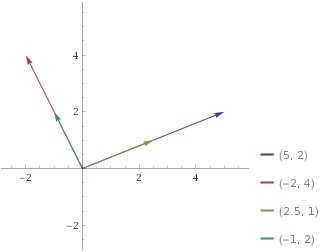
\includegraphics{vectors1}
            \centering
            \par}
            \\\\
            
            \\If we pick any vector $\vec{x}=\begin{bmatrix} x_1\\x_2\end{bmatrix}$ then:
            
            $$
             \operatorname{T}(\vec{x})=\begin{bmatrix} 0.5 & 0 \\ 0 & 0.5\end{bmatrix} \begin{bmatrix} x_1\\x_2 \end{bmatrix}
            = x_1 \begin{bmatrix} 0.5\\0\end{bmatrix} + x_2 \begin{bmatrix} 0\\0.5\end{bmatrix}
            = \begin{bmatrix} 0.5x_1\\0\end{bmatrix} + \begin{bmatrix} 0\\0.5x_2\end{bmatrix}
            = \begin{bmatrix}0.5x_1 \\ 0.5x_2 \end{bmatrix}
            $$
            
            This transformation is geometrically scaling the vectors by a factor of two, basically halving each vector in length while maintaining direction.
            
            \subsection*{Problem 16}
            
            $$
            \operatorname{T}(\vec{x})=\begin{bmatrix} 0 & 1 \\ 1 & 0\end{bmatrix} \begin{bmatrix} x_1\\x_2 \end{bmatrix}
            $$
            \operatorname{T}(\vec{u})=\begin{bmatrix} 0 & 1 \\ 1 & 0\end{bmatrix} \begin{bmatrix} 5\\2 \end{bmatrix}
            = 5 \begin{bmatrix} 0\\1\end{bmatrix} + 2 \begin{bmatrix} 1\\0\end{bmatrix}
            = \begin{bmatrix} 0\\5\end{bmatrix} + \begin{bmatrix} 2\\0\end{bmatrix}
            = \begin{bmatrix}2 \\ 5 \end{bmatrix}
            $$\\\\
            $$\\
             \operatorname{T}(\vec{v})=\begin{bmatrix} 0 & 1 \\ 1 & 0\end{bmatrix} \begin{bmatrix} -2\\4 \end{bmatrix}
            = -2 \begin{bmatrix} 0\\1\end{bmatrix} + 4 \begin{bmatrix} 1\\0\end{bmatrix}
            = \begin{bmatrix} 0\\-2\end{bmatrix} + \begin{bmatrix} 4\\0\end{bmatrix}
            = \begin{bmatrix}4 \\ -2 \end{bmatrix}
            
            \\\\
            {\centering 
            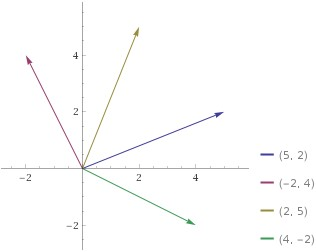
\includegraphics{vectors2}
            \centering
            \par}
            \\\\
            
            \\If we pick any vector $\vec{x}=\begin{bmatrix} x_1\\x_2\end{bmatrix}$ then:
            
            $$
             \operatorname{T}(\vec{x})=\begin{bmatrix} 0 & 1 \\ 1 & 0\end{bmatrix} \begin{bmatrix} x_1\\x_2 \end{bmatrix}
            = x_1 \begin{bmatrix} 0\\1\end{bmatrix} + x_2 \begin{bmatrix} 1\\0\end{bmatrix}
            = \begin{bmatrix} 0\\x_1\end{bmatrix} + \begin{bmatrix} x_2\\0\end{bmatrix}
            = \begin{bmatrix}x_2 \\ x_1 \end{bmatrix}
            $$
            
            This transformation is geometrically scaling reflecting the vectors around the line $x_1=x_2$ (analogous to $y=x$ in the $(x, y)$ plane).
        
\end{document}
